%--------------------
% Packages
% -------------------
\documentclass[11pt,a4paper]{article}
\title{Spatial Context Influence on Cell Type Classification}
\author{Amelia Lockley, Stella Messenger, Tuan Tran, Eva Cheng,  ChengCheng Ye}
\date{May 31th - 2026}
\usepackage[utf8x]{inputenc}
\usepackage[T1]{fontenc}
%\usepackage{gentium}
\usepackage{mathptmx} % Use Times Font

\usepackage[pdftex]{graphicx} % Required for including pictures
\usepackage[pdftex,linkcolor=black,pdfborder={0 0 0}]{hyperref} % Format links for pdf
\usepackage{calc} % To reset the counter in the document after title page
\usepackage{enumitem} % Includes lists

\frenchspacing % No double spacing between sentences
\linespread{1.2} % Set linespace
\usepackage[a4paper, lmargin=0.1666\paperwidth, rmargin=0.1666\paperwidth, tmargin=0.1111\paperheight, bmargin=0.1111\paperheight]{geometry} %margins
\usepackage{parskip}

\usepackage[all]{nowidow} % Tries to remove widows
\usepackage[protrusion=true,expansion=true]{microtype} % Improves typography, load after fontpackage is selected

\usepackage{fancyhdr} % Adds the DATA3888 header to each page
\pagestyle{fancy}
\fancyhf{} % Clear existing header/footer settings
\fancyhead[R]{DATA3888 Group Report}
\fancyfoot[C]{\thepage} 
\usepackage{enumitem} % Required for custom labels
\usepackage{adjustbox}
\usepackage{natbib} % https://www.overleaf.com/learn/latex/Bibliography_management_with_natbib
\usepackage{multirow}
\usepackage{booktabs}
\usepackage{float}
\usepackage{caption}
\usepackage{graphicx}
\captionsetup{font=footnotesize}
\bibliographystyle{apalike} % Makes bibliography in APA format

%-----------------------
% Begin document
%-----------------------
\begin{document} 
\maketitle
\section{Executive Summary}

The past diagnosis of breast cancer diagnosis usually relied on the manual interpretation of haematoxylin and 
eosin (H\&E) stained tissue images by expert pathologists --- a process that is time-consuming and subject to inter-observer variability \citep{elmore2015}. This study investigates whether deep learning models can automatically classify breast cancer cell subtypes from H\&E image patches, and specifically examines how the amount of surrounding spatial context captured in each patch affects classification performance. 

Using single-cell H\&E image patches derived from a Xenium in situ sequencing dataset \citep{janesick2023}, we trained and evaluated three deep learning models 
--- ResNet-50, Vision Transformer (ViT), and CTransPath --- on a three-class classification task: Invasive Tumor, DCIS\_1, and DCIS\_2. Each model was trained under three experimental conditions: full context (100 pixel patches), reduced context 
(50 pixel patches), and minimal context (masked patches retaining only the central 30\% 
of the image).

Our findings demonstrate that spatial context richness improves H\&E-based 
classification of breast cancer cell subtypes, with performance consistently 
decreasing as context was reduced. However, cell types defined by transcriptomic 
rather than morphological criteria --- such as Prolif\_Invasive\_Tumor and 
Invasive\_Tumor --- cannot be reliably distinguished from images alone, limiting 
the applicability of this approach to subtypes with distinct histological features.

These findings highlight the importance of spatial context in H\&E-based cell 
type classification, resulting in the creation of a Shiny web application which allows clinical researchers 
and cancer biologists to interactively explore model predictions across different 
context conditions.

\section{Introduction}
\subsection{Background and Motivation}

Breast cancer tissue is highly heterogeneous, with tumour progression influenced not only by the morphology of individual cells, but also by the surrounding tumour microenvironment (TME). In clinical pathology, spatial relationships between tumour cells, stromal regions, immune infiltration, and tissue boundaries are often critical for diagnosis and prognosis. However, many traditional single-cell approaches rely on tissue dissociation, which removes this spatial information and limits the ability to analyse how cells interact within their native environment.

Recent advances in spatial transcriptomics and in situ imaging suggest that preserving tissue context is important for accurately identifying tumour cell subtypes. \cite{janesick2023} showed that certain tumour populations and “boundary cells” were difficult to distinguish once spatial positioning within the tissue was lost. This is particularly relevant in breast cancer, where the distinction between ductal carcinoma in situ (DCIS) and invasive tumour regions is strongly associated with tissue-level structural organisation rather than isolated cellular morphology alone.

Despite the growing use of deep learning in computational pathology, it remains unclear how much surrounding tissue context contributes to subtype classification performance, as many models focus primarily on local morphological features while larger-scale tissue architecture is less well understood. Understanding this relationship is important for developing more robust and clinically interpretable pathology models.

\subsection{Study Aim and Hypothesis}

This study investigates how varying levels of spatial context influence deep learning-based classification of breast cancer tumour subtypes from H\&E histology images using the Xenium dataset \cite{janesick2023}. We hypothesise that richer spatial context will improve classification performance, particularly for subtypes whose distinction depends on tissue architecture rather than individual cell morphology.

\section{Methods}

\begin{figure}[H]
    \centering
    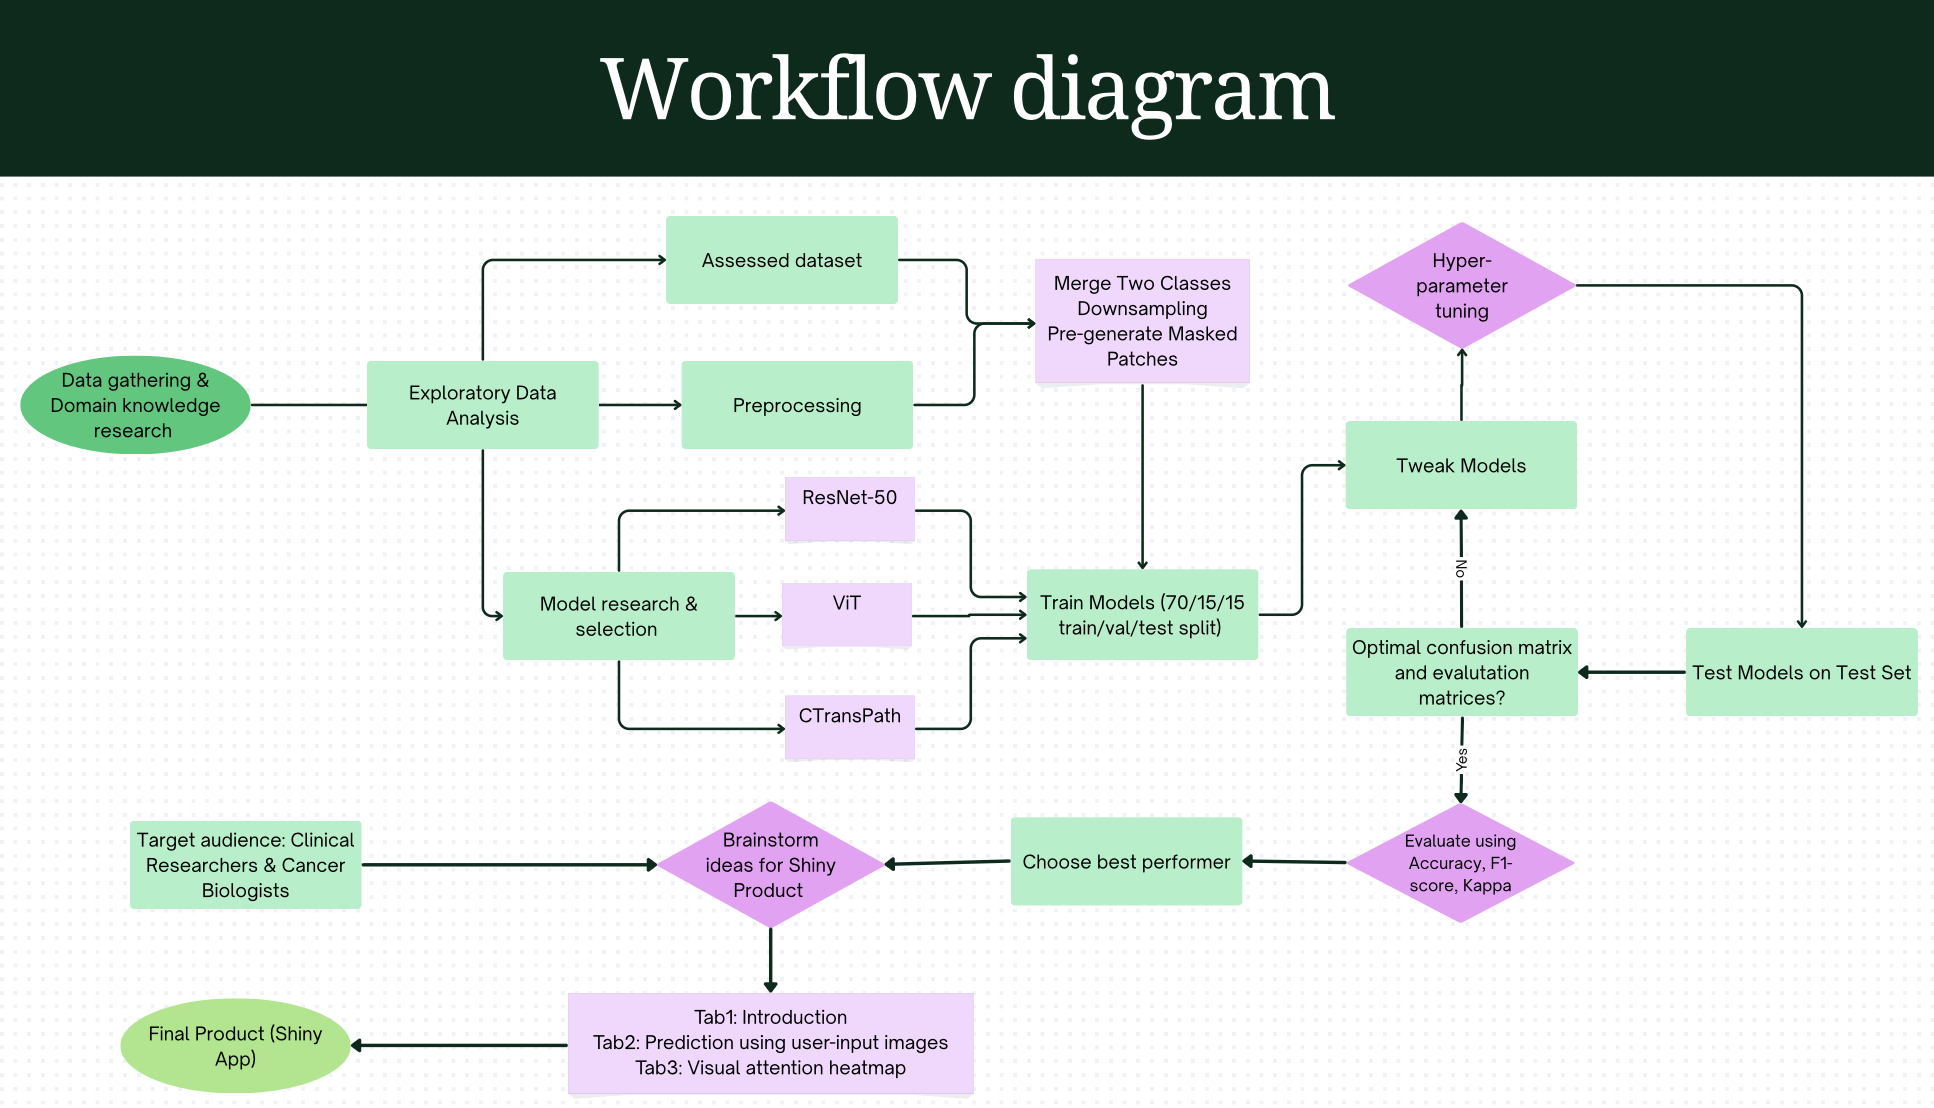
\includegraphics[width=\textwidth]{images/workflow_diagram.png}
    \label{fig:wf_diagram}
    \caption{Workflow Diagram}
\end{figure}

\subsection{Exploratory Data Analysis}

\subsubsection{Dataset Overview}

    The dataset is derived from \cite{janesick2023}, who profiled a formalin-fixed paraffin-embedded (FFPE) human breast cancer tissue section using the Xenium in situ platform. Cell identity labels were assigned through integration of scRNA-seq data with spatial transcriptomic information, yielding 20 distinct cell types spanning tumour epithelial, immune, stromal, and myoepithelial populations.
    
\begin{figure}[H]
    \centering
    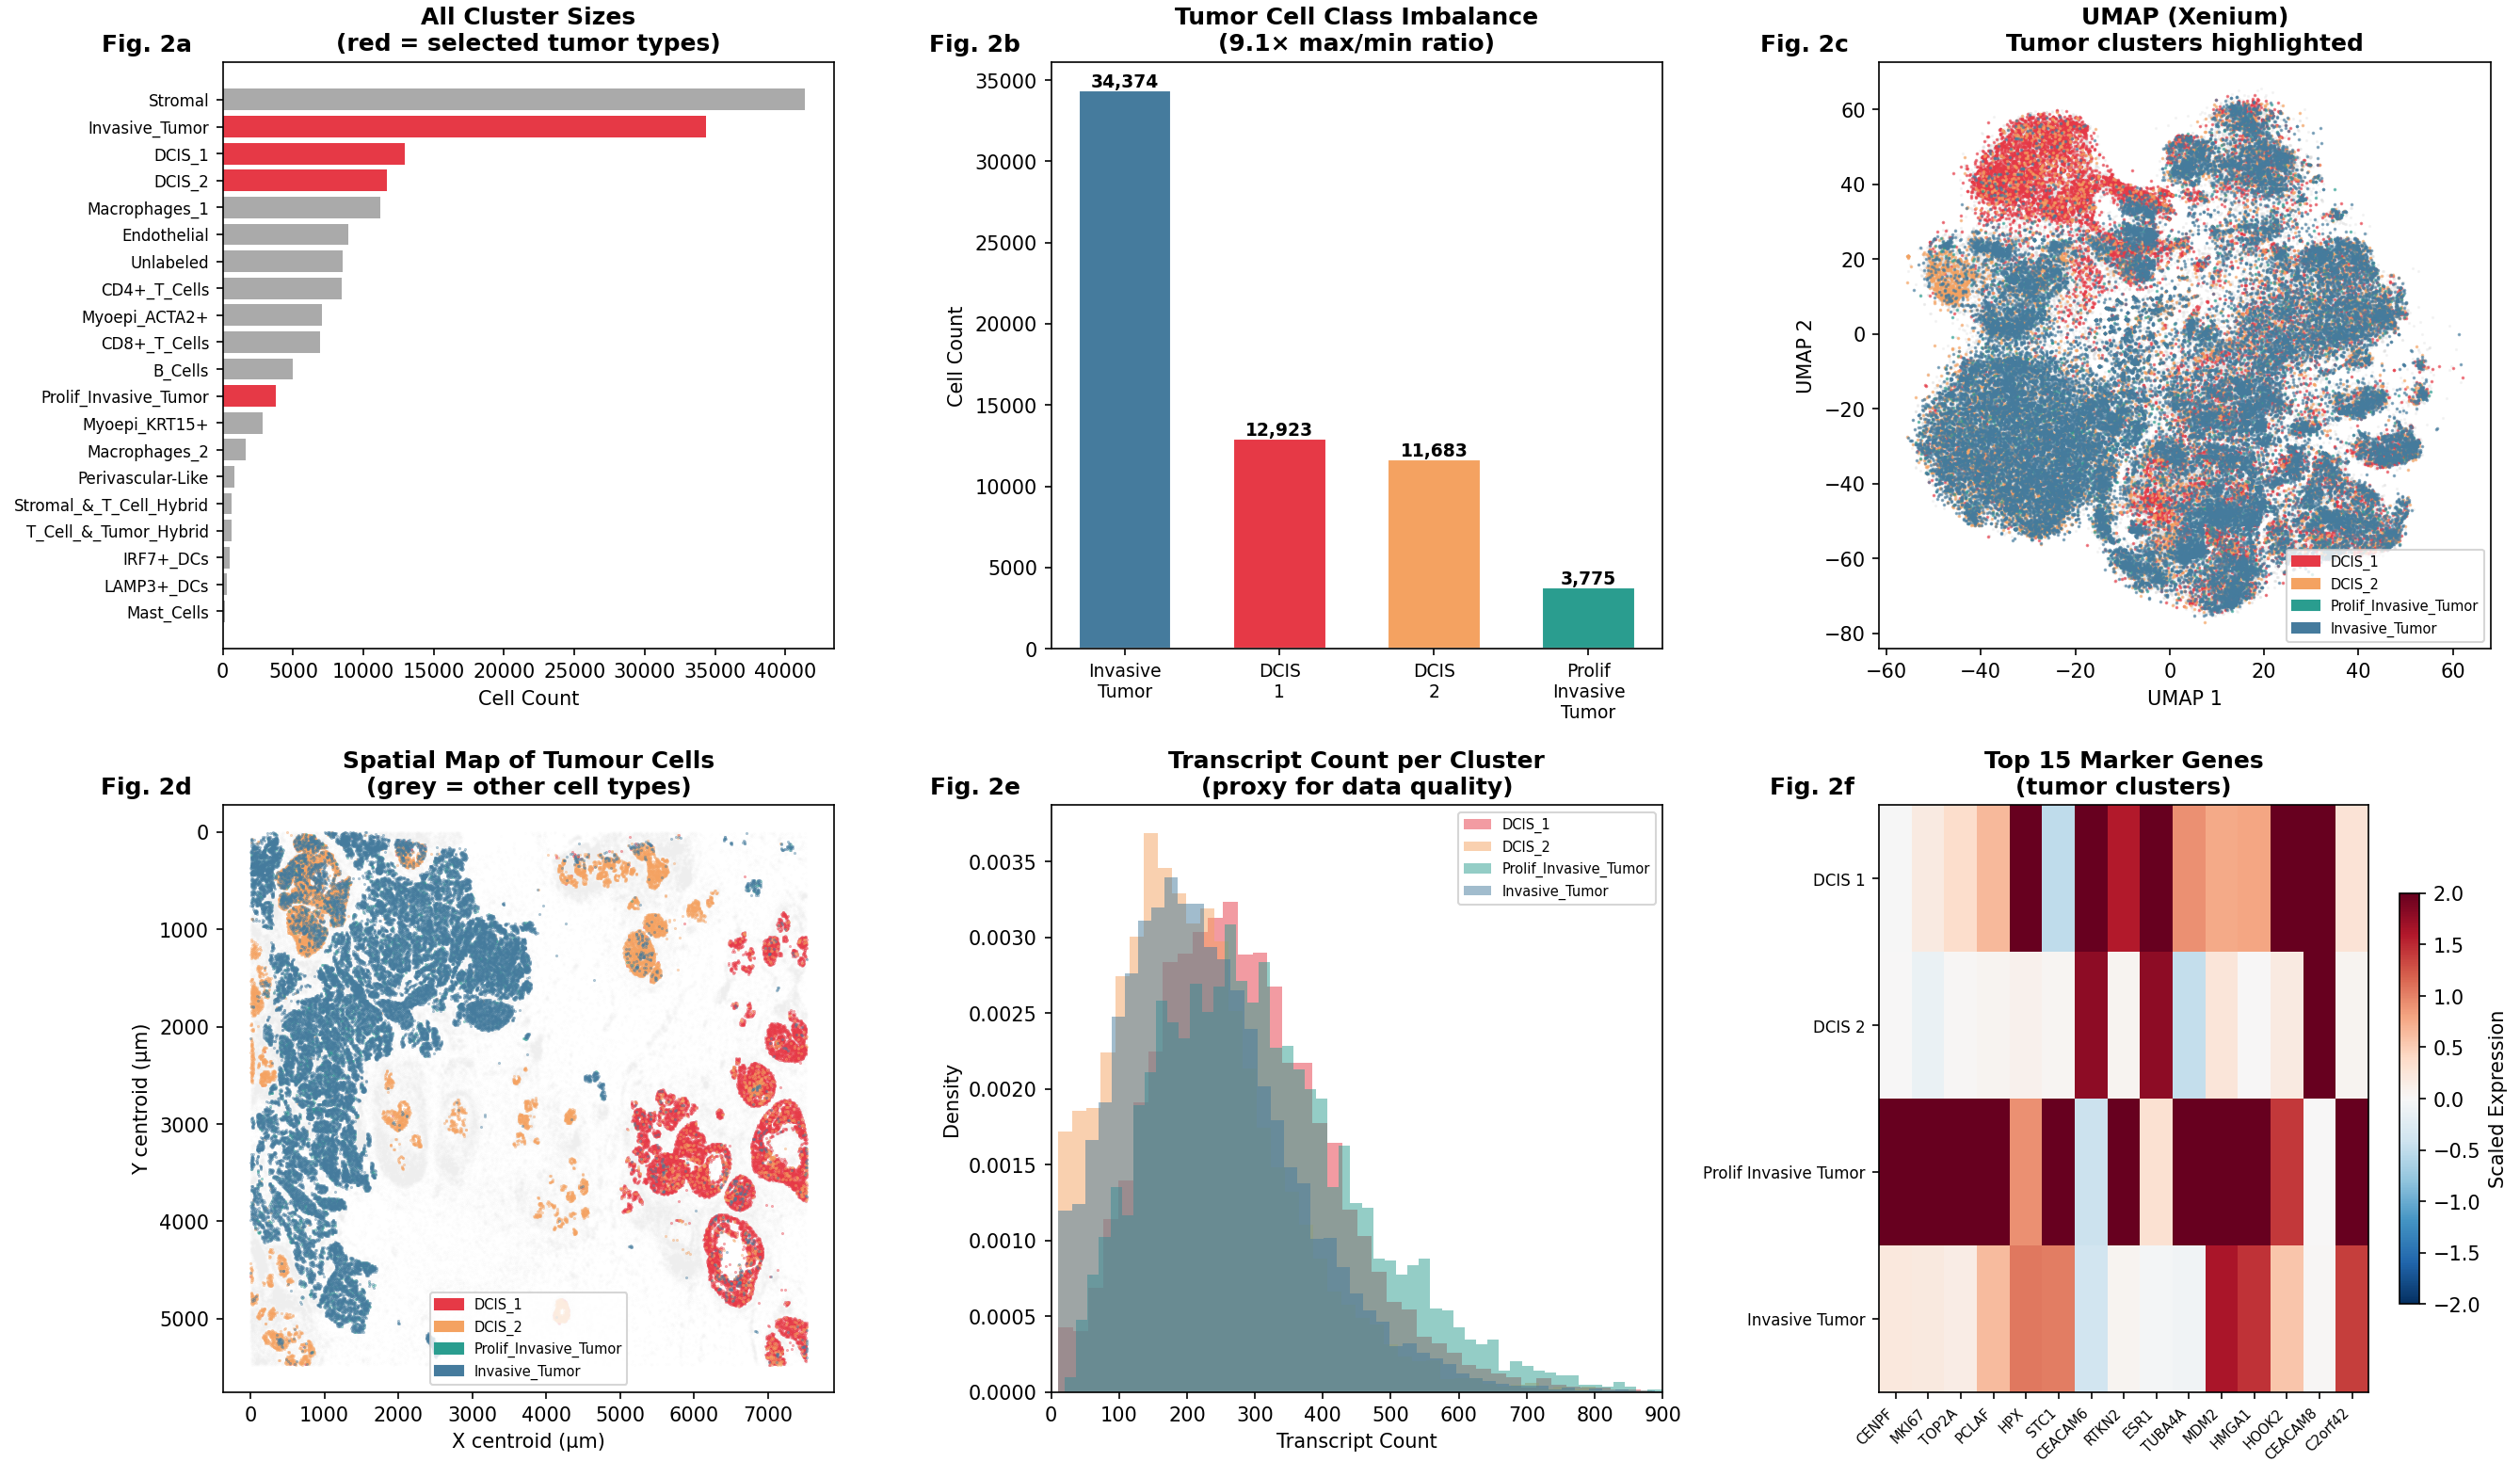
\includegraphics[width=\textwidth]{images/fig1_eda_overview.png}
    \caption{Exploratory data analysis of the Xenium breast cancer dataset.}
\end{figure}

Figure. 2a provides a spatial overview of the dataset. As shown in Figure. 2b, the dataset exhibits substantial class imbalance, with \textit{Invasive\_Tumor} comprising 34,374 cells compared to only 3,775 \textit{Prolif\_Invasive\_Tumor} cells (9.1$\times$ ratio). Figure. 2e shows comparable transcript count distributions across all four subtypes, indicating consistent data quality. Figure .2c and Figure .2f together indicate that \textit{Prolif\_Invasive\_Tumor} and \textit{Invasive\_Tumor} are highly similar at the molecular level, occupying overlapping regions in transcriptomic space with near-identical marker gene expression. Figure.2d further confirms that these two subtypes are spatially intermixed within the tissue section with no clear boundary.

\subsubsection{Morphological Separability Analysis}

To assess whether the four tumour subtypes are visually distinguishable from H\&E images alone, we conducted a morphological separability analysis comparing cell-level image features across all class pairs.

Visual inspection of H\&E patches reveals that while DCIS\_1 and DCIS\_2 occupy spatially distinct regions within the tissue, Prolif\_Invasive\_Tumor and Invasive\_Tumor cells are spatially intermixed with no clear morphological boundary. This result is consistent with the study by \citet{janesick2023}.

\begin{figure}[H]
    \centering
    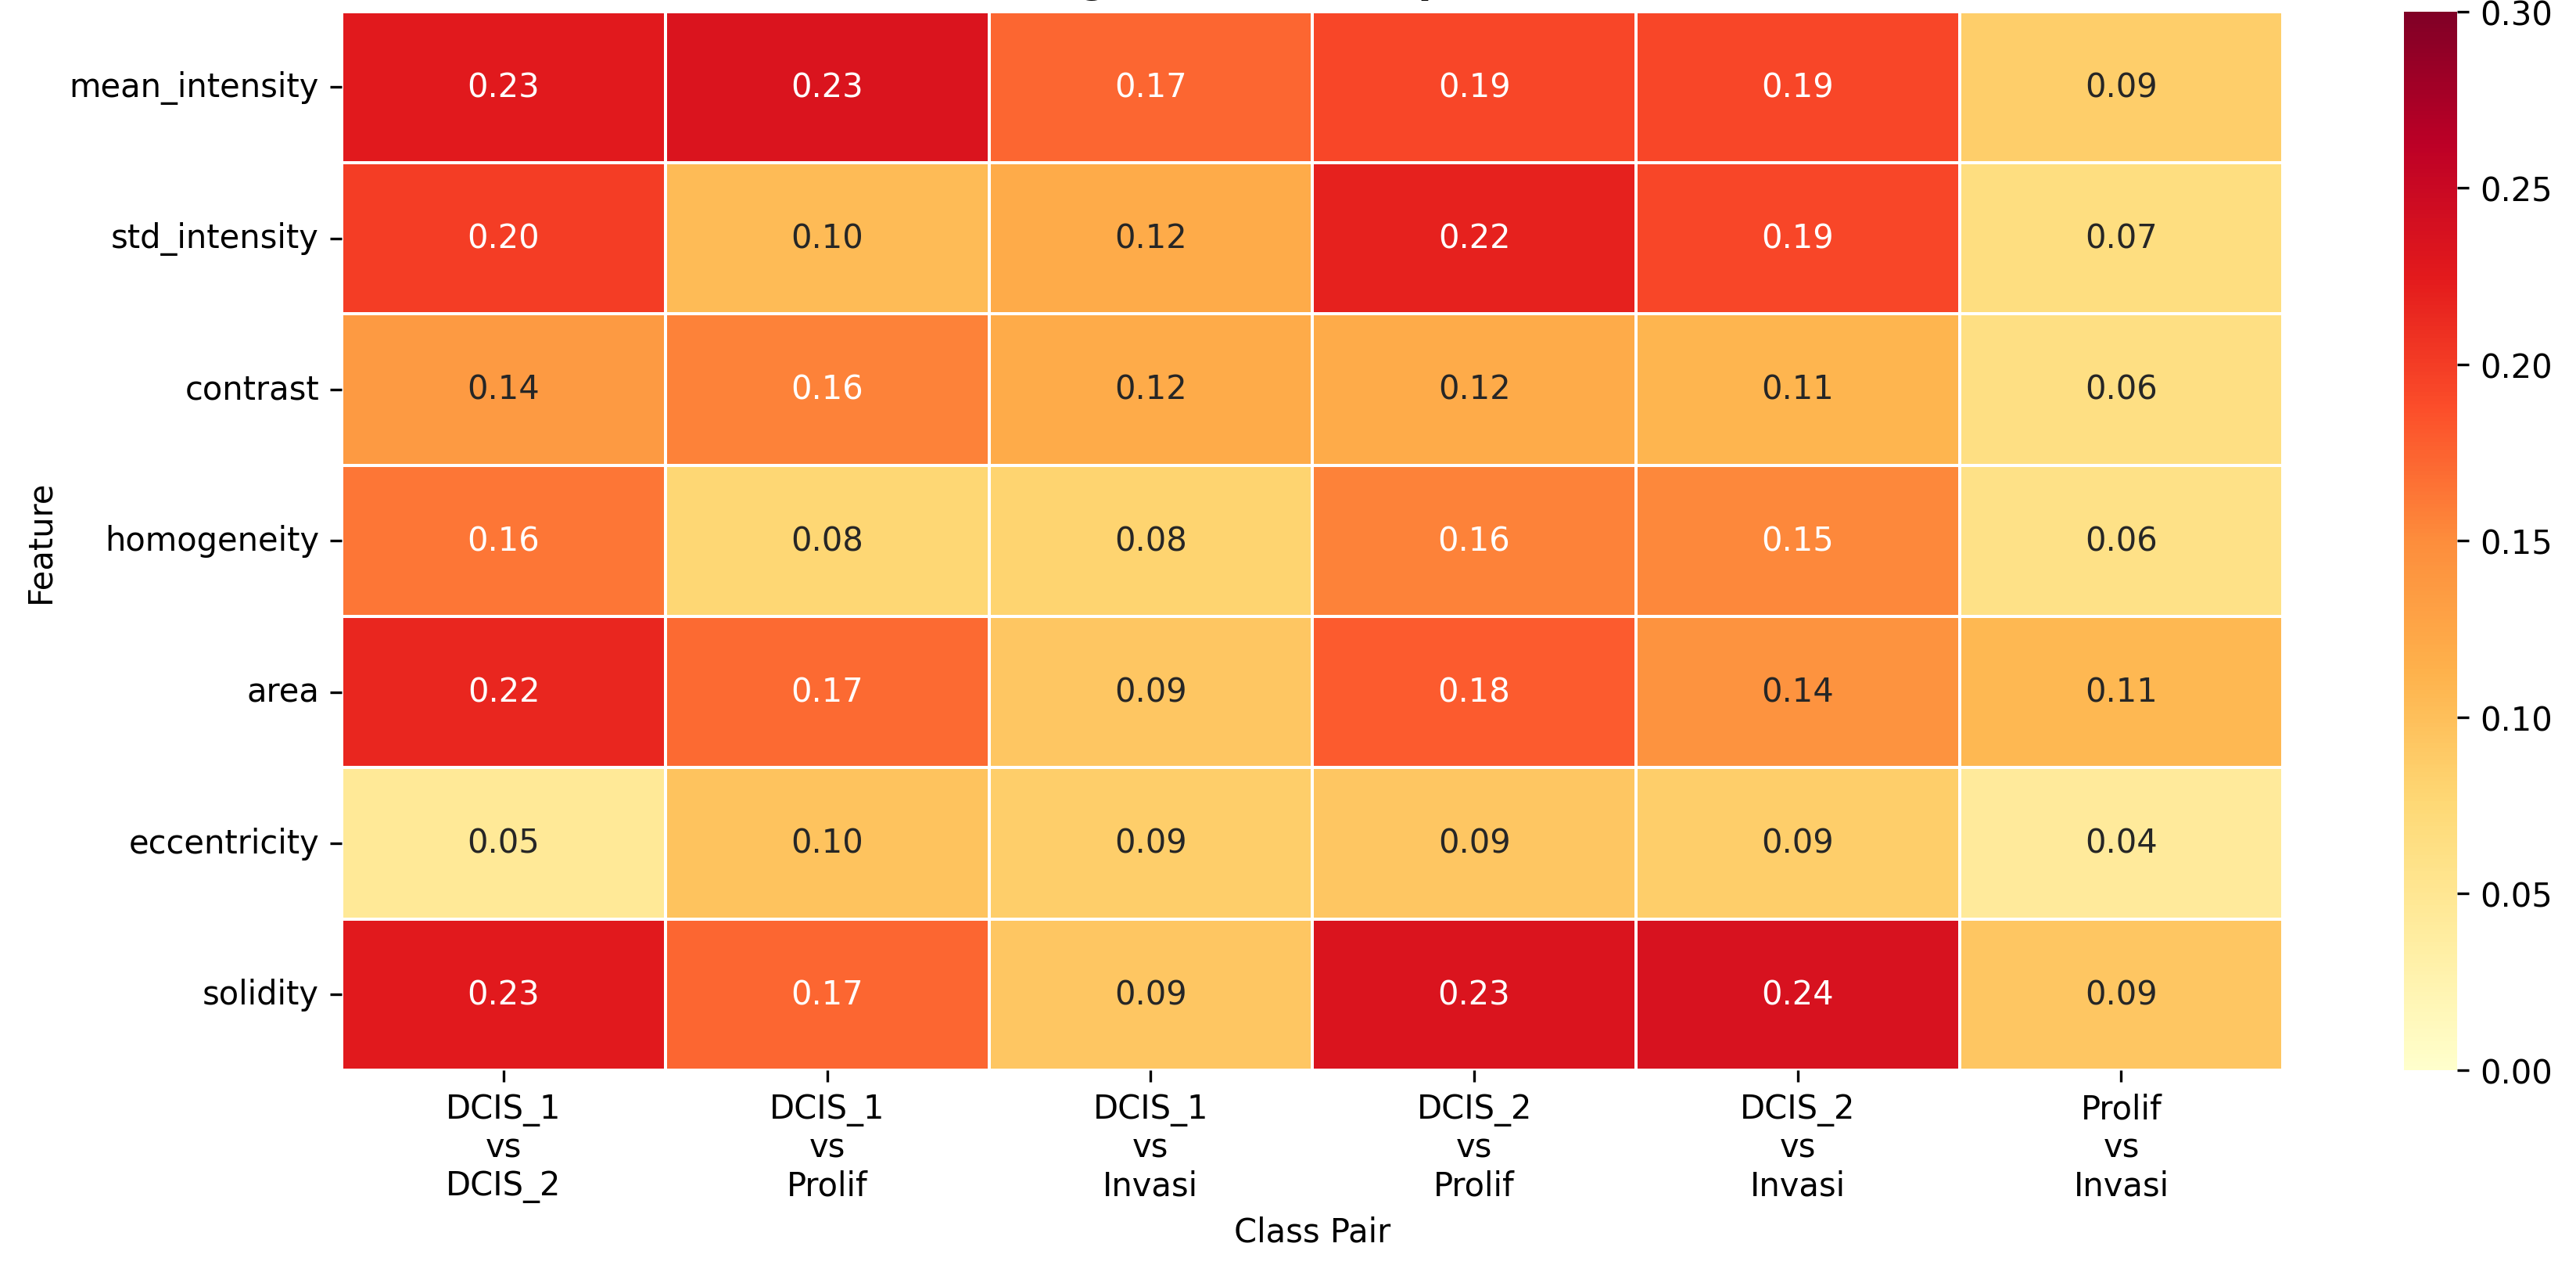
\includegraphics[width=\textwidth]{images/ks_heatmap.png}
    \caption{KS statistic heatmap comparing morphological feature distributions across all tumour subtype pairs.}
\end{figure}

To quantify this observation, we computed the Kolmogorov-Smirnov (KS) statistic between each class pair across seven morphological features: mean intensity, standard deviation of intensity, contrast, homogeneity, area, eccentricity, and solidity. The KS statistic measures the difference between two distributions, where higher values indicate greater separability. As shown in Figure3, the Prolif vs Invasive pair consistently yields the lowest KS values across all features (range: 0.04--0.11), substantially lower than other class pairs. This confirms that Prolif\_Invasive\_Tumor and Invasive\_Tumor are not separable based on morphological image features alone.
    
\subsection{Preprocessing}

\subsubsection{Rationale for Class Merging}

    Based on the morphological separability analysis, Prolif\_Invasive\_Tumor and 
    Invasive\_Tumor are indistinguishable from H\&E images alone, as both subtypes are 
    defined by scRNA-seq clustering rather than histological criteria \citep{janesick2023}. They were therefore merged into a single Tumor class, yielding a three-class classification task: Tumor, DCIS\_1, and DCIS\_2.

\subsubsection{Class Imbalance and Downsampling}

    Following the merging of Prolif\_Invasive\_Tumor and Invasive\_Tumor, the three classes remain imbalanced. To ensure balanced training, each class was downsampled to 10,000 samples. For the Tumor class, all 3,775 available Prolif\_Invasive\_Tumor samples were retained, with the remaining 6,225 samples drawn from Invasive\_Tumor. DCIS\_1 and DCIS\_2 were each randomly downsampled to 10,000 respectively, yielding a final dataset of 30,000 cells across three balanced classes.

\subsubsection{Train/Validation/Test Split}

The dataset was partitioned into training, validation, and test sets using a stratified random split of 70/15/15. Stratification was applied on the class label to ensure a consistent class distribution across all three splits. The final split yielded 21,000 training samples, 4,500 validation samples, and 4,500 test samples prior to spatial leakage removal.

\subsubsection{Spatial Leakage Removal}

To prevent data leakage arising from overlapping image patches, test cells were filtered based on their spatial proximity to training and validation cells. Using a BallTree structure on the Xenium centroid coordinates, any test cell within a 10µm radius of a train or validation cell was excluded. Following this procedure, the test set was reduced from 4,500 to 2,879 cells, with approximately 36\% of test cells removed.

\subsubsection{Masked Patch Generation}

To isolate the contribution of spatial context, masked versions of each image patch were generated. A circular mask was applied to each patch, retaining only the central 30\% of the image radius and filling the surrounding region with the ImageNet mean grey value (RGB: 123, 116, 103). This produced a masked variant for each cell that preserves only the central cell morphology while removing surrounding tissue context, enabling a comparison between full-context and context-free classification conditions.

\subsubsection{Normalisation Statistics}

Per-channel mean and standard deviation were computed from a random sample of 1,000 training images and applied during preprocessing across all three experimental conditions.

\subsection{Experimental Design}

    The experimental design is a 3 by 3 factorial setup, which uses three architectures to represent different modelling philosophies: local convolutional features, global attention, and a pathology‑specific local-global hybrid. Factor 1 consists of different context conditions: nucleus‑only (masked), 50 pixel, 100 pixel and factor 2 is the model family: ResNet‑50, ViT, CTransPath.

    For each combination, we train a separate model on the same training data and evaluate on the same held‑out test set. This design allows us to compare, within a model family, how changing context affects performance and, within a context level, whether certain architectures exploit context more effectively than others.

\subsection{Model development}

\subsubsection{ResNet-50}

ResNet-50 is a 50-layer convolutional neural network with residual connections, enabling 
effective training of deep networks \citep{he2016deep}. It applies convolutional blocks 
with increasing channel depth and decreasing spatial resolution, followed by global 
average pooling and a fully connected classification layer.

The model was initialised with ImageNet-pretrained weights. The final layer was replaced 
with a three-class output head with dropout ($p = 0.5$). Only \texttt{layer4} and the 
classification head were unfrozen for fine-tuning, with differential learning rates 
($3 \times 10^{-4}$ for the head, $3 \times 10^{-5}$ for \texttt{layer4}) and L2 
regularisation (weight decay $= 10^{-2}$).

ResNet-50 was selected as a strong and widely used baseline in computational pathology, 
providing a benchmark against which more specialised architectures could be compared.

\subsubsection{Vision Transformer (ViT)}
    The Vision Transformer (ViT) is a transformer‑based image classifier that views an image as a sequence of non-overlapping fixed‑size patches (similar to tokens in natural language processing) \citep{dosovitskiy2021, wu2020}. Each patch is linearly embedded and combined with positional encodings, and the sequence is processed by a standard Transformer encoder using multi‑head self‑attention. ViT models are unlike CNNs as they focus more on global and long-range patterns \citep{wu2020}, which may be especially relevant when broader tissue context is important. 
    
    We elected to implement ViT models as one of our experiments as ViT explicitly models global relationships, so it is a good test of whether attention‑based architectures benefit more from larger context (100 pixel) than from more restricted views (50 pixel, nucleus‑only).
    
    We used “google/vit-base-patch16–224” model, which is pre-trained on ImageNet-21k and fine-tuned on ImageNet 2012 \citep{huggingface2021,dosovitskiy2021}. We replaced the classification head with a four‑class linear layer and fine-tuned all layers on each of the three input conditions.\


\subsubsection{CTransPath} 

    CTransPath by \cite{WANG2022102559} is a model built specifically for analysing histopathology images. It first uses convolutional layers to pick up small-scale visual details in an H\&E image patch, such as edges, cell boundaries, and fine texture. It then uses a transformer-based component to combine information across a wider area of tissue, helping it capture both local cell appearance and broader tissue structure efficiently.

    The model was first trained on millions of pathology image patches without needing manual labels. Because of this large-scale pretraining on histology data, it learns image features that are especially well-suited to H\&E morphology.

    In our study, we reused this pre‑trained backbone and added a small task‑specific classification head on top. The backbone outputs a 768‑dimensional vector for each input patch; we feed this into a series of fully connected layers that reduce the representation to a three‑dimensional output, corresponding to the three breast cancer cell subtypes of interest. Training proceeds in two steps: we first train only the new head while keeping the backbone frozen, which lets the classifier learn how to interpret the existing features without immediately altering them. We then unfreeze the backbone and fine‑tune the entire network, but with a lower learning rate for the backbone than for the head, so that the rich histopathology features learned from large pre-training data are only gently adjusted to our Xenium‑derived breast cancer patches.

\subsection{Evaluation Strategy}

Model performance was assessed using three primary quantitative metrics: \textit{accuracy}, to capture overall predictive performance; \textit{macro F1}, to evaluate performance equally across all cell subtypes, including minority classes; and \textit{Cohen’s kappa}, to quantify agreement between predictions and ground truth beyond chance expectations under the observed class distribution.

Additionally, we chose to run McNemar's test on the models. McNemar's test allows for direct model to model comparison. Using a 2x2 contingency table, it tallies the number of images:
\begin{enumerate}[label=(\alph*)]
    \item Correctly classified by both Model 1 and Model 2;
    \item Incorrectly classified by both Model 1 and Model 2;
    \item Incorrectly classified by Model 1; and
    \item Incorrectly classified by Model 2
\end{enumerate}

The test helps determine whether the counts in categories \textit{(c)} and \textit{(d)} differ more than expected by chance. The null hypothesis being: \textit{"both models have the same probability of correctly classifying an image"}. By conducting this test on every pair of model experiments, we are able to identify differences in accuracy that are statistically significant.

\section{Results}

\begin{figure}[H]
    \centering
    %\begin{adjustbox}{center}
    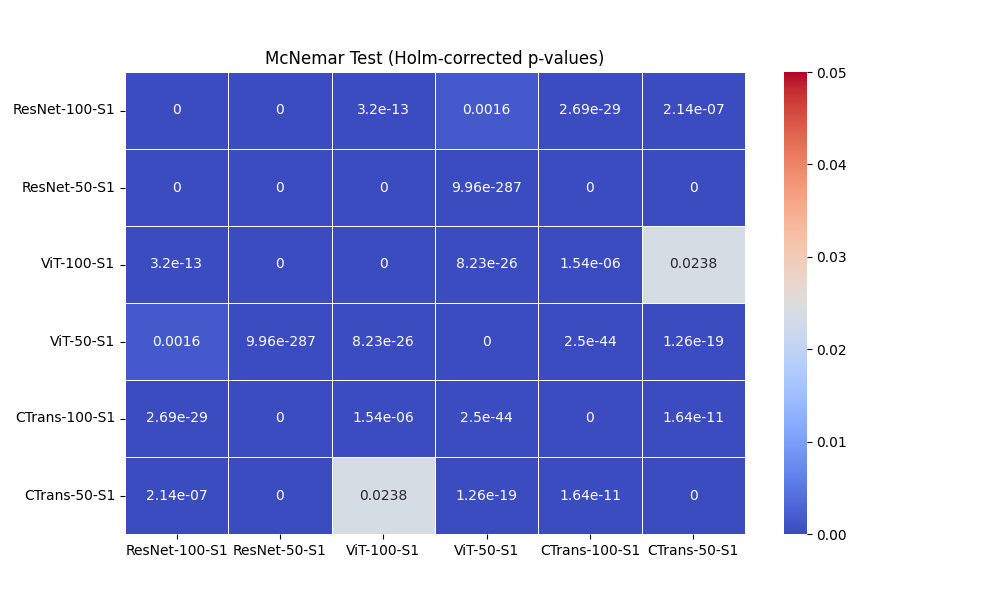
\includegraphics[width=\textwidth]{images/McNemar.png}
    %\end{adjustbox}
    \caption{McNemar's Heatmap with adjusted p-values using Holm correction to control family-wise error rate (due to multiple pairwise comparisons). \textit{\textbf{N.B.} masked models were evaluated on a larger dataset, and thus could not be compared to other models using McNemar's test.}}
    \label{fig:mcnemar}
\end{figure}

\subsection{General Insights}
We found that, in general, all models had their performance increase as their spatial context increased. Table~\ref{tab:models} shows an average increase of 10 percentage points in accuracy from the models trained on masked images versus the models trained on the full 100 pixel context. This is further made evident through Figure~\ref{fig:tab3}, with an example of a cell having its most attention-heavy areas at around 100 pixel away from the centre.

The pattern of the positive effect of spatial context in performance is further reinforced in Figure~\ref{fig:mcnemar}. Nearly all model comparisons have adjusted p-values that indicated that the null hypothesis should be rejected. This indicated that the changes seen in the accuracy of the models are statistically significant and are unlikely to be due to random variation.

However, in Figures 6, 7, 8, reveal consistently low accuracy for certain cell types regardless of context condition. This reflects a fundamental limitation: when cell type identity is defined transcriptomically rather than morphologically \citep{janesick2023}, histologically indistinguishable subtypes cannot be reliably separated by image-based models alone.

% The increase in focus on these areas, and the strengthening of evaluation metrics, indicates that the greater spatial information provided meaningful data in the models' basis for classification labelling. 


% im done with it btw, so u can make changes here now

\begin{table}[ht]
\centering
\begin{adjustbox}{center}
\begin{tabular}{llcccccc}
\toprule
 &  & \textbf{Accuracy} & \textbf{Macro F1} & \textbf{Kappa} & \multicolumn{3}{c}{\textbf{F1 Score}} \\
\cmidrule(lr){6-8}
\textbf{Model} & \textbf{Spatial Context} &  &  &  & \textbf{Tumour} & \textbf{DCIS 1} & \textbf{DCIS 2} \\
\midrule
\multirow[t]{3}{*}{ResNet-50} & 100px & 92.0 & 91.5 & 87.8 & 94.7 & 92.8 & 87.1 \\
 & 50px & 85.1 & 83.8 & 77.1 & 82.2 & 83.9 & 84.2 \\
 & Masked & 80.4 & 80.5 & 70.7 & 81.9 & 83.1 & 76.5 \\
\cline{1-8}
\multirow[t]{3}{*}{ViT} & 100px & 94.3 & 93.9 & 91.3 & 96.7 & 94.5 & 90.4 \\
 & 50px & 90.7 & 90.2 & 85.9 & 93.5 & 91.6 & 85.6 \\
 & Masked & 81.2 & 81.2 & 71.8 & 83.4 & 84.2 & 75.8 \\
\cline{1-8}
\multirow[t]{3}{*}{CTransPath} & 100px & 95.2 & 94.9 & 92.8 & 97.2 & 95.4 & 92.0 \\
 & 50px & 93.7 & 93.2 & 90.4 & 96.4 & 94.1 & 89.2 \\
 & Masked & 89.4 & 89.3 & 84.0 & 91.9 & 90.5 & 85.4 \\
\cline{1-8}
\bottomrule
\end{tabular}
\end{adjustbox}
\caption{Model comparison results}
\label{tab:models}
\end{table}

\subsection{Final Model}
For our final product, we selected CTransPath, which had the comparatively best evaluation metrics in all spatial context settings(Table~\ref{tab:models}). In addition to having the highest accuracy, macro F1 and Cohen's kappa scores, CTransPath showed the most minimal differences class-wise performance, especially for DCIS 2, which was consistently challenging across all model types. This lead to an overall stronger performance for the model. Furthermore, as discussed above, McNemar's test (Figure~\ref{fig:mcnemar}) indicated that many of the performance differences between CTransPath and other models were statically significant, which further supported our selection of it for our final product.

\subsection{Deployment Process}

Using the chosen CTransPath model, we developed an interactive Python Shiny dashboard to support cancer biologists and clinical researchers in exploring how spatial context influences cell-type classification. The first tab (Figure~\ref{fig:tab1}) briefly explains the dataset and the chosen model, along with instructions on using the next tabs. 

The second tab (Figures~\ref{fig:dc2_tab2}, \ref{fig:dc1_tab2}, \ref{fig:tum_tab2}) allows users to insert image patches in 100 pixel, 50 pixel or 30\% masked versions and see what they were classified as by the model. Beneath each inserted image, the predicted probabilities for the three tumour subtypes (Tumour, DCIS\_1, and DCIS\_2) are shown, enabling users to directly assess how classification changes as spatial context is reduced. 

The third tab (Figure~\ref{fig:tab3}) showcases attention visualisation and provides a qualitative indication of which image regions contributed most strongly to model predictions under each spatial context condition. For each patch uploaded in the previous tab, the dashboard provides an attention heatmap overlay highlighting the image regions most influential to the model’s prediction. This helps users relate the model’s behaviour to meaningful histological structures, such as duct boundaries or densely packed cell clusters.

\section{Discussion and Conclusion}

\subsection{Limitations}

\subsubsection{Dataset}

The current dataset was derived from a single tissue section, which may introduce patient-specific or staining-batch biases and therefore limit the generalisability of the findings. In addition, some tumour subtypes are underrepresented in the dataset, which may reduce the stability and reliability of performance estimates for minority classes.

There is also a risk of patch overlap, as spatially adjacent patches may share background information across training and test splits. To minimise this form of data leakage, stricter spatial deduplication procedures or validation on independent patient samples would be required.

Finally, the current evaluation is largely confined to a single tissue section. Broader assessment across multiple patients, multiple centres, and cross-validation settings is still needed to establish the robustness and external validity of the models.

\subsubsection{Modelling}

    CTransPath was originally pre-trained on much larger tissue regions, such as whole-slide image tiles, rather than single-cell patches. As a result, this shift from tile-level to cell-level features may reduce how effectively the learned representations transfer to the present task.

    In addition, the classifier head is relatively simple, relying on a single global average of spatial features. While this provides a compact representation, it also removes positional information about where discriminative features are located within the patch.
    
    Finally, because the task involves only three classes and a relatively small dataset derived from a single tissue section, there is a risk that the model captures patient-specific tissue characteristics rather than broadly generalisable cell morphology.
    
\subsection{Conclusion}

This study demonstrates that spatial context plays a critical role in the classification of breast cancer cell types. Models that incorporate a broader surrounding tissue region achieve more stable and consistent classification performance, suggesting that the local tissue architecture around a cell provides important information for model decision-making.

The interactive interface developed in this project further supports this finding by allowing researchers to visually compare model predictions under different spatial-context conditions. In doing so, it offers a practical tool for examining and interpreting how the model responds to changes in the amount of surrounding tissue information.

Overall, this work provides a foundation for the development of more interpretable and clinically relevant pathology models that are sensitive to spatial context. It also establishes a basis for future studies involving larger, multi-patient and multi-centre datasets.

\section{Student Contribution}

\begin{itemize}
    \item \textbf{\textit{Amelia Lockley: }} Responsible for conducting exploratory data analysis, developing and refining the final version of Shiny App Tab 2, redesigning the Shiny application user interface, and writing the Introduction section of the report.
    \item \textbf{\textit{Stella Messenger: }} Responsible for development and fine-tuning of the ViT models. Additionally, responsible for running the comparison of all trained models. Wrote evaluation strategies and results sections 1 \& 2, and revised the ViT description in the report.
    \item \textbf{\textit{Tuan Tran: }} Responsible for finetuning the CTransPath model under all mentioned experimental conditions, documenting the code repository, and finalising the report. 
    \item \textbf{\textit{Eva Cheng: }} Defined the research topic, experimental framework, and project structure. Conducted EDA and implemented the full preprocessing pipeline, including the masked patch experiment design. Fine-tuned ResNet-50 and ViT models. Developed Shiny app Tab 1 and Tab 2. Responsible for the EDA, preprocessing, and ResNet-50 methodology sections of the report.
    \item \textbf{\textit{ChengCheng Ye: }}  Responsible for the implementation of the functions of the two versions of tab3, the completion of tab1 in the initial version, and also finished the writing of the relevant part about the Shiny app in the report.
\end{itemize}
\newpage
\bibliographystyle{apalike}
\bibliography{references}
\newpage
\section{Appendix}

\begin{figure}[H]
    \centering
    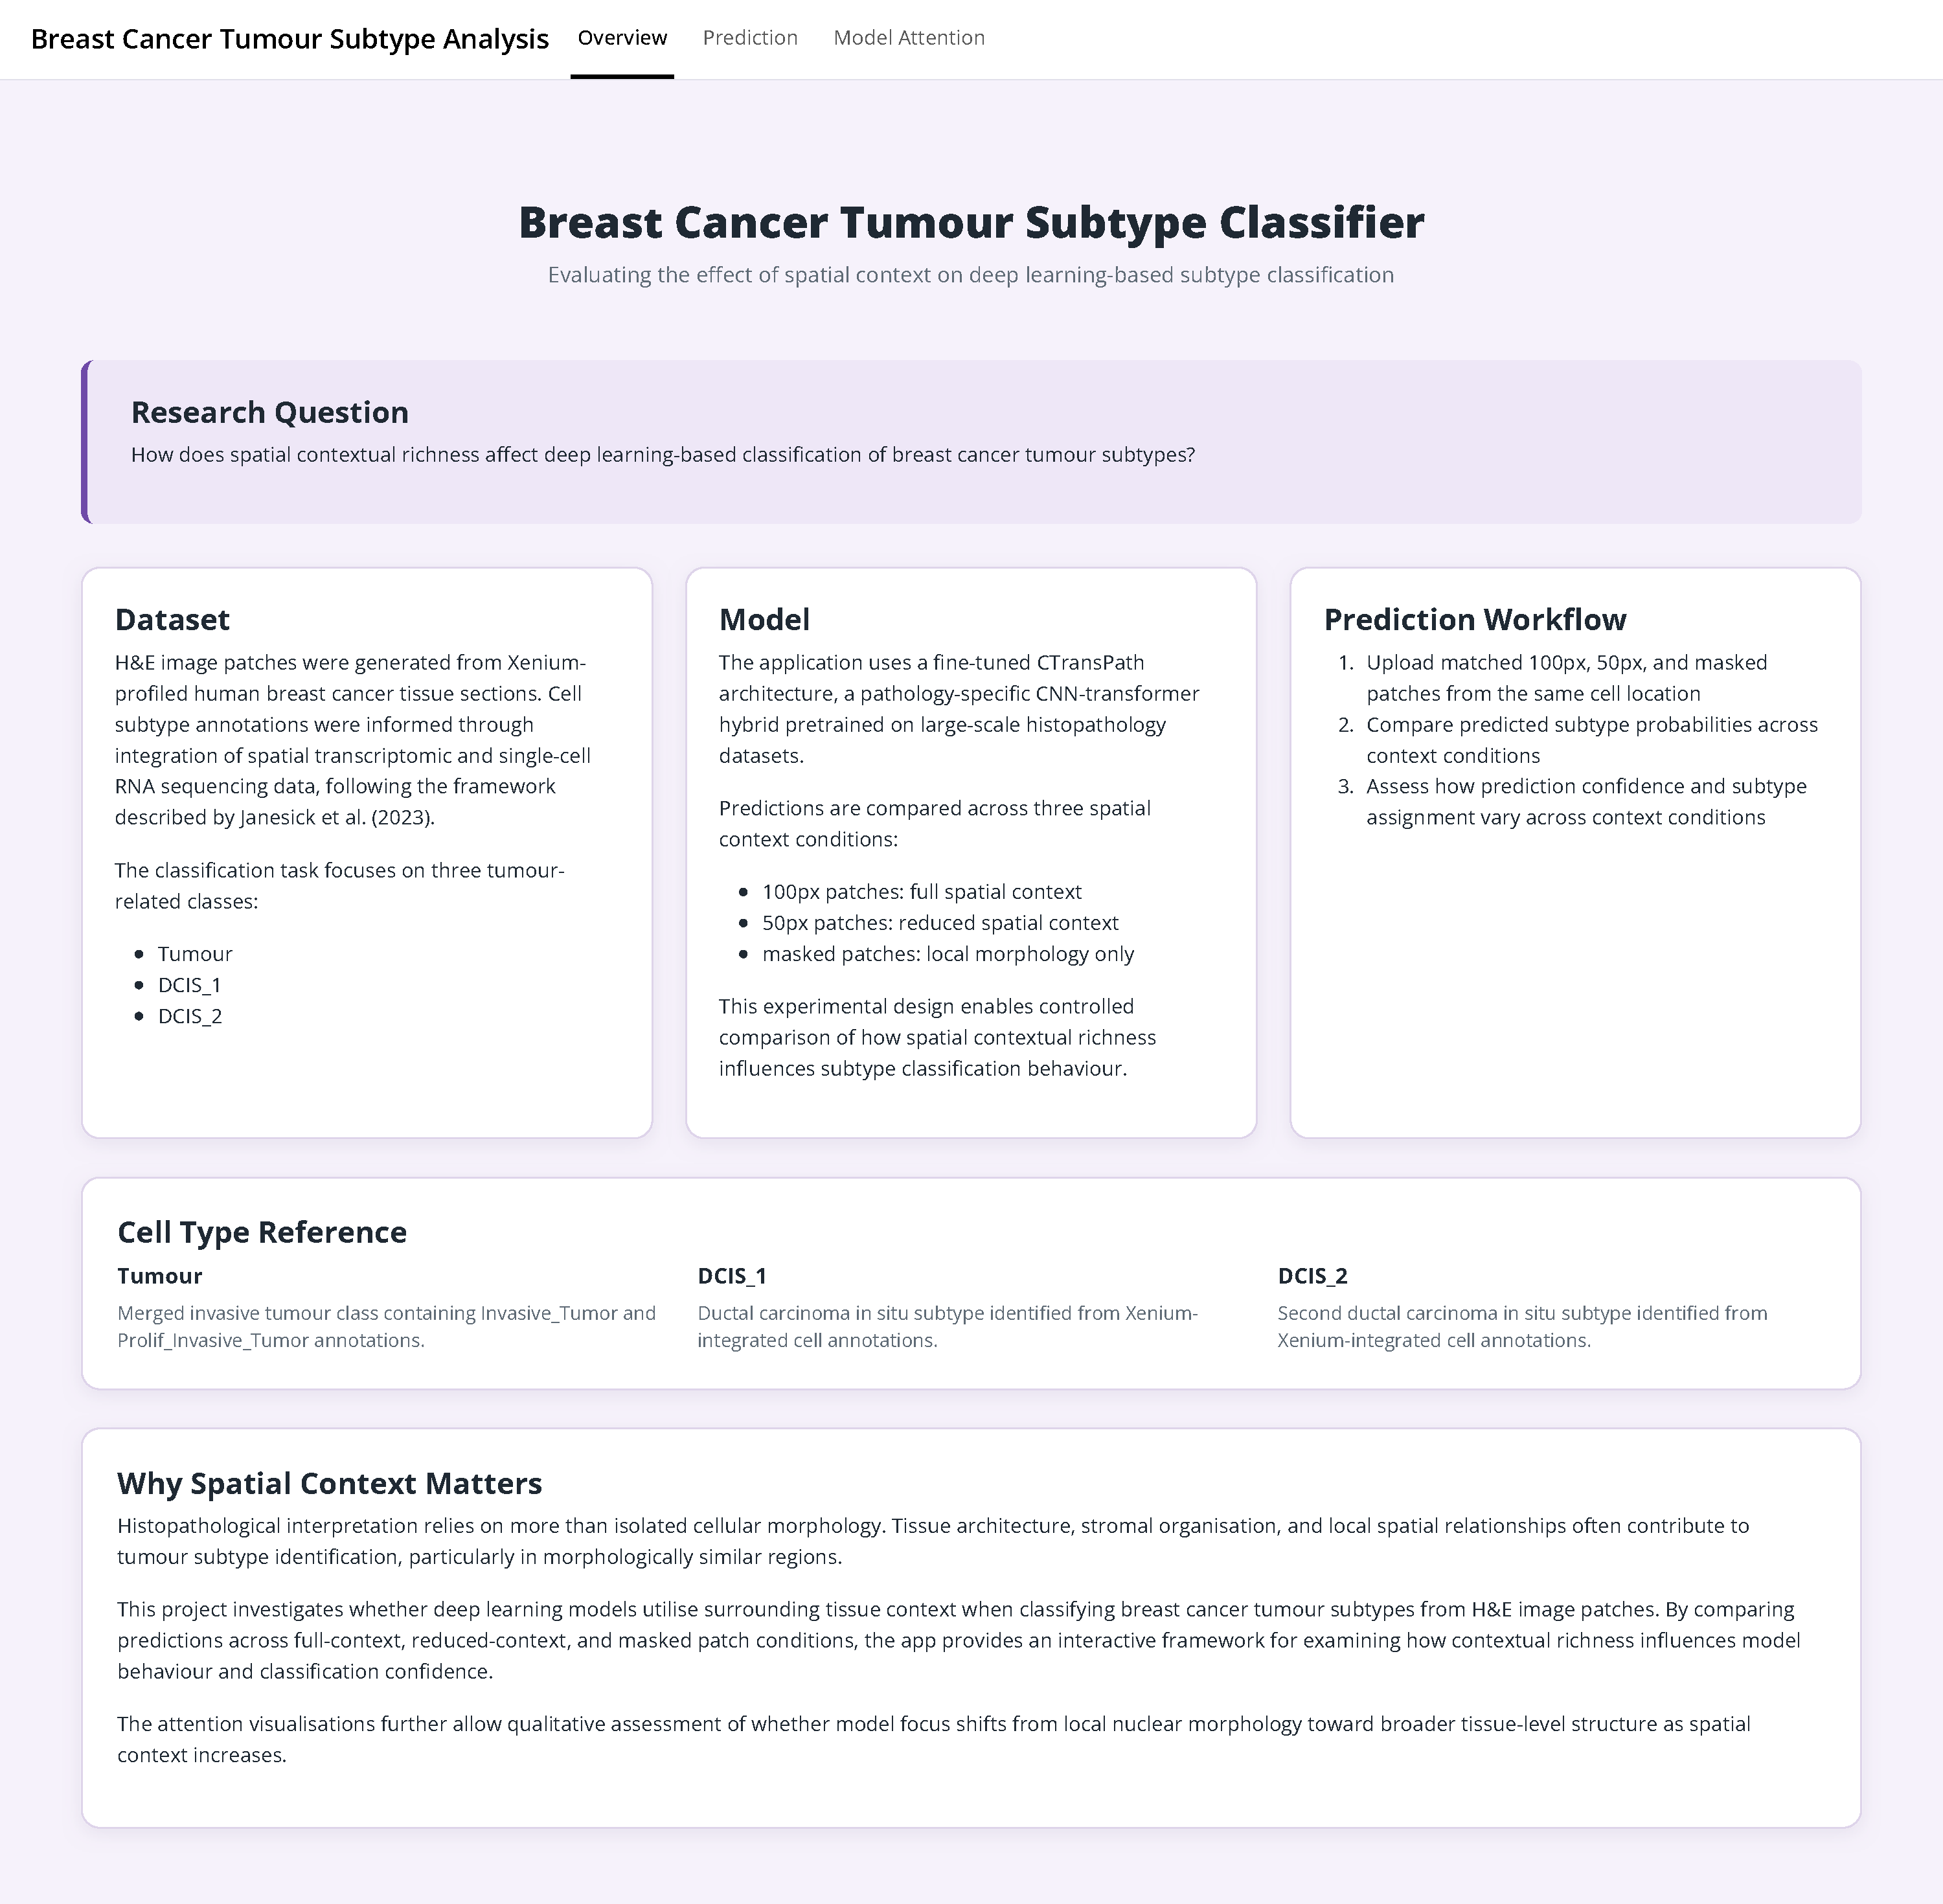
\includegraphics[width=\textwidth]{images/Breast Cancer Tumour Subtype Analysis}
    \caption{Tab 1: Breast Cancer Tumour Subtype Analysis Introduction Page}
    \label{fig:tab1}
\end{figure}

\begin{figure}[H]
    \centering
    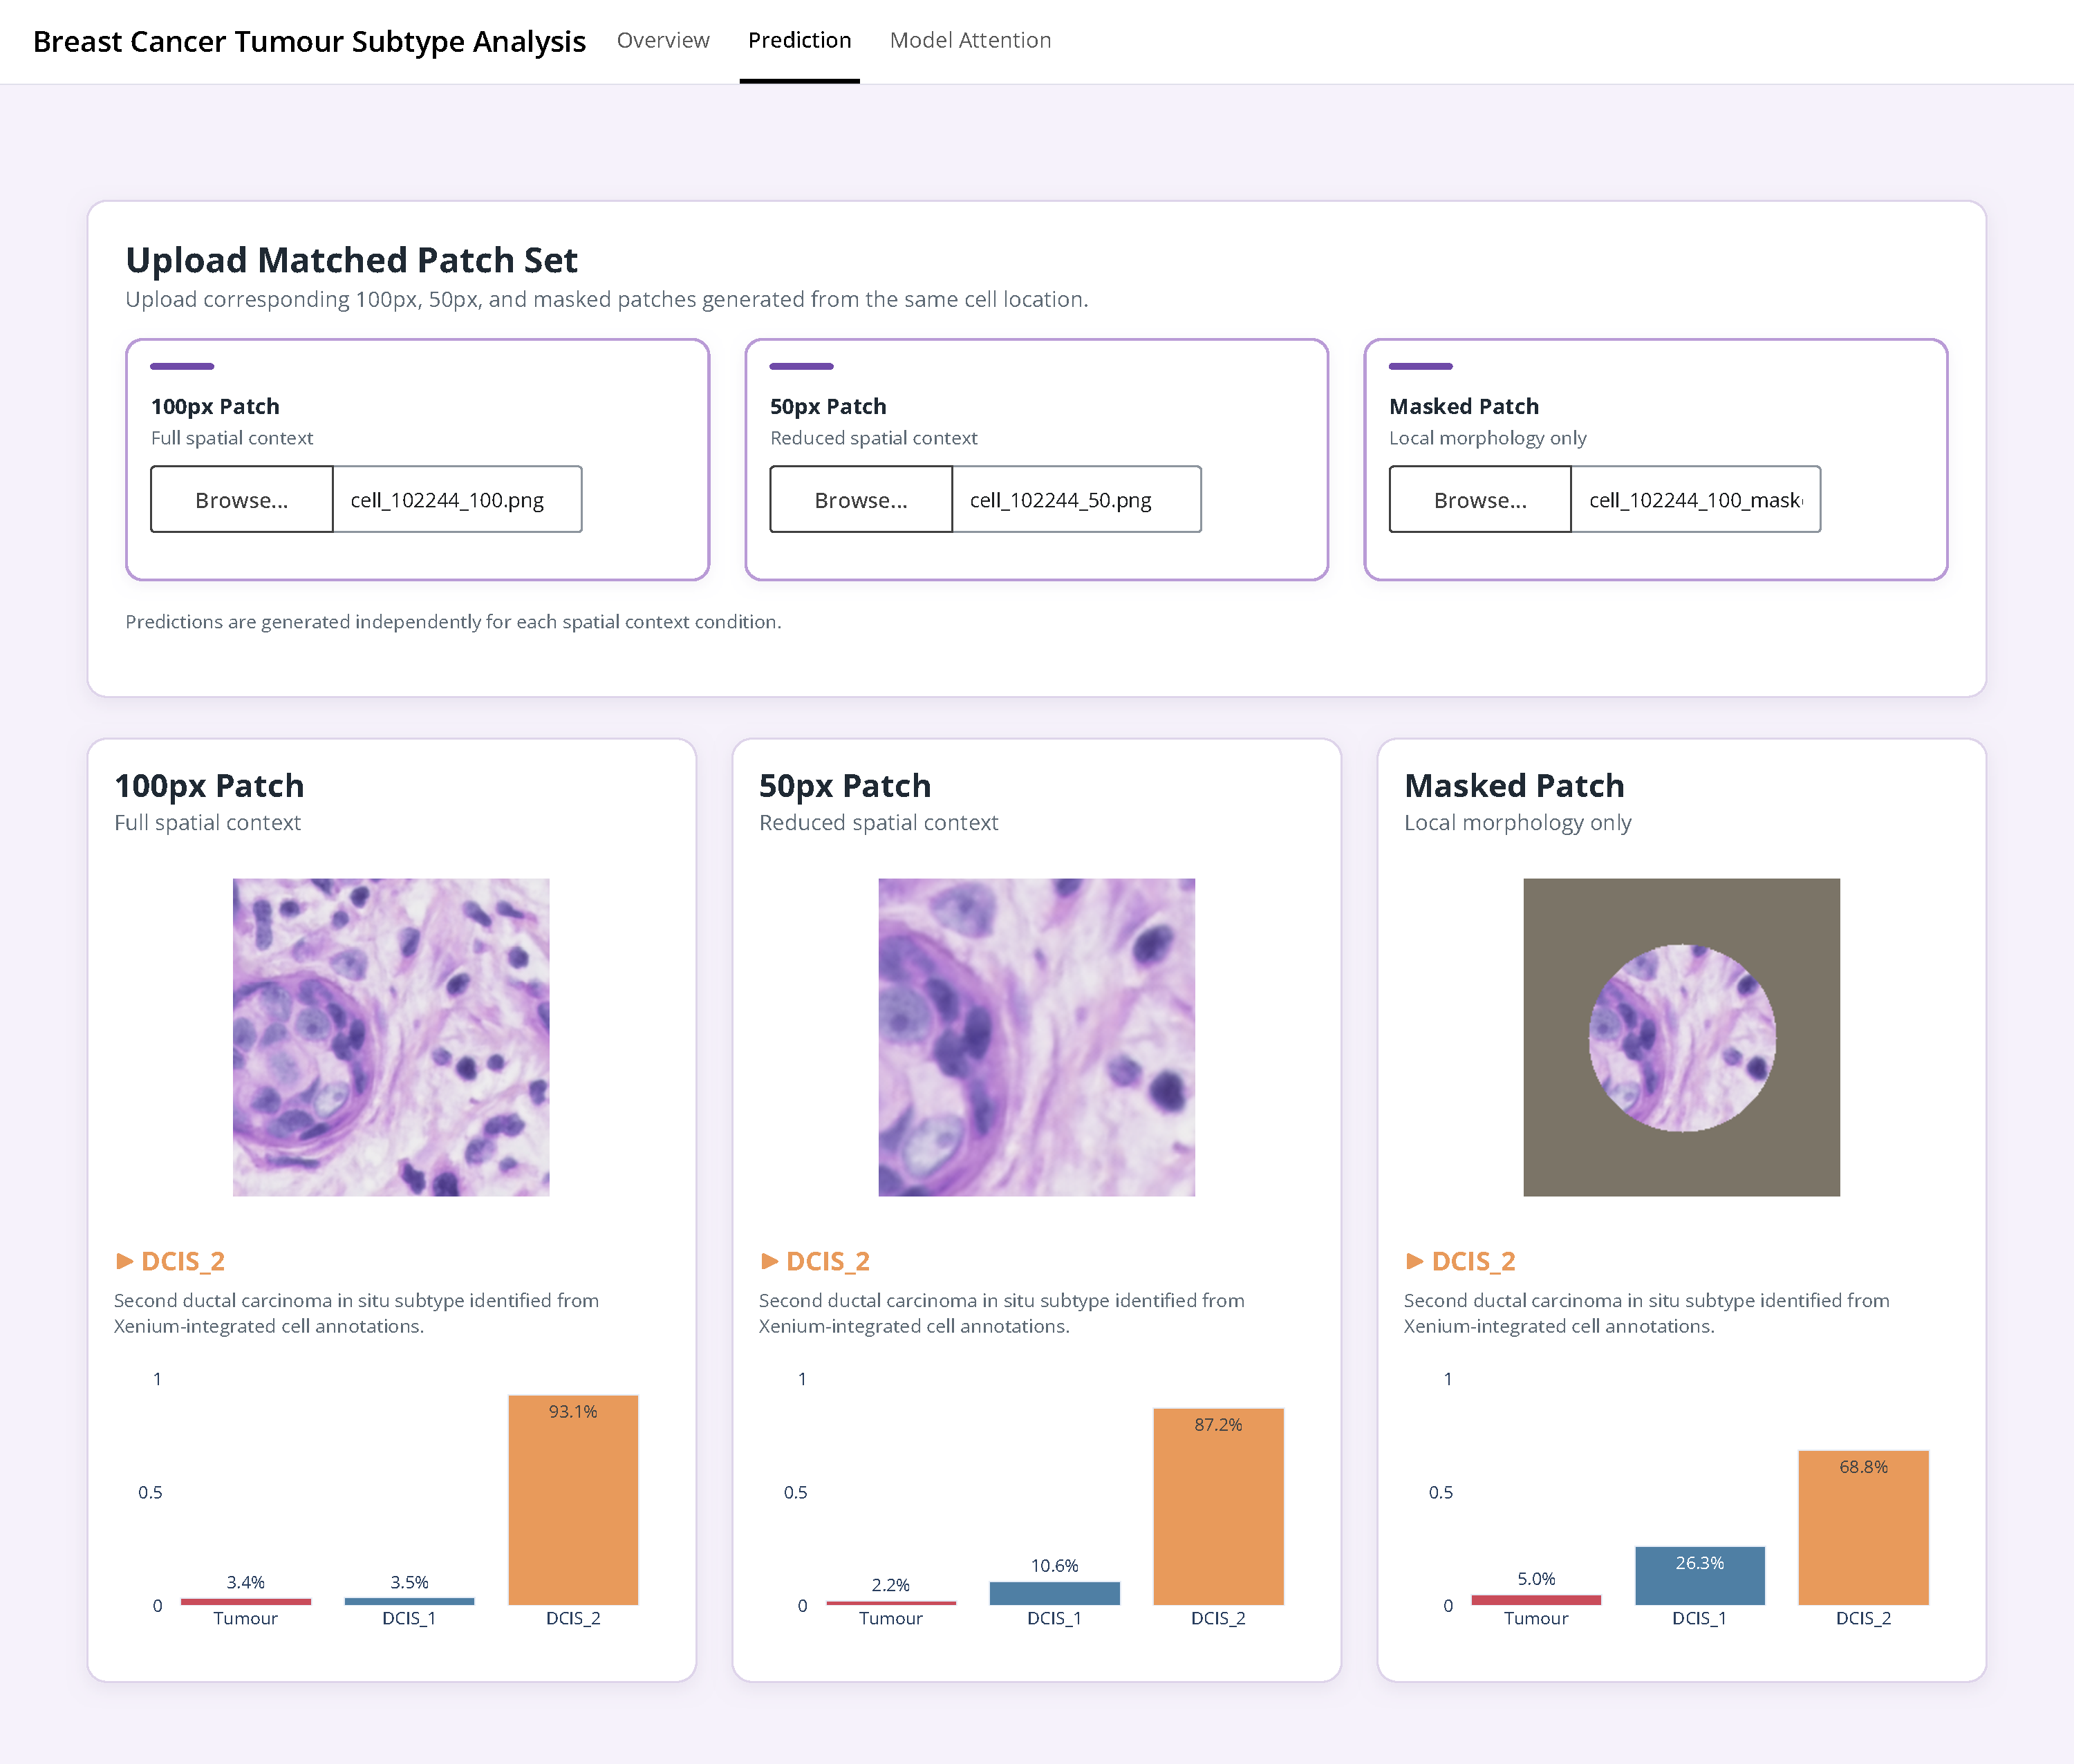
\includegraphics[width=\textwidth]{images/Breast Cancer Tumour Subtype Analysis Cell type prediction}
    \caption{Tab2 : Prediction for cell\_102244}
    \label{fig:dc2_tab2}
\end{figure}

\begin{figure}[H]
    \centering
    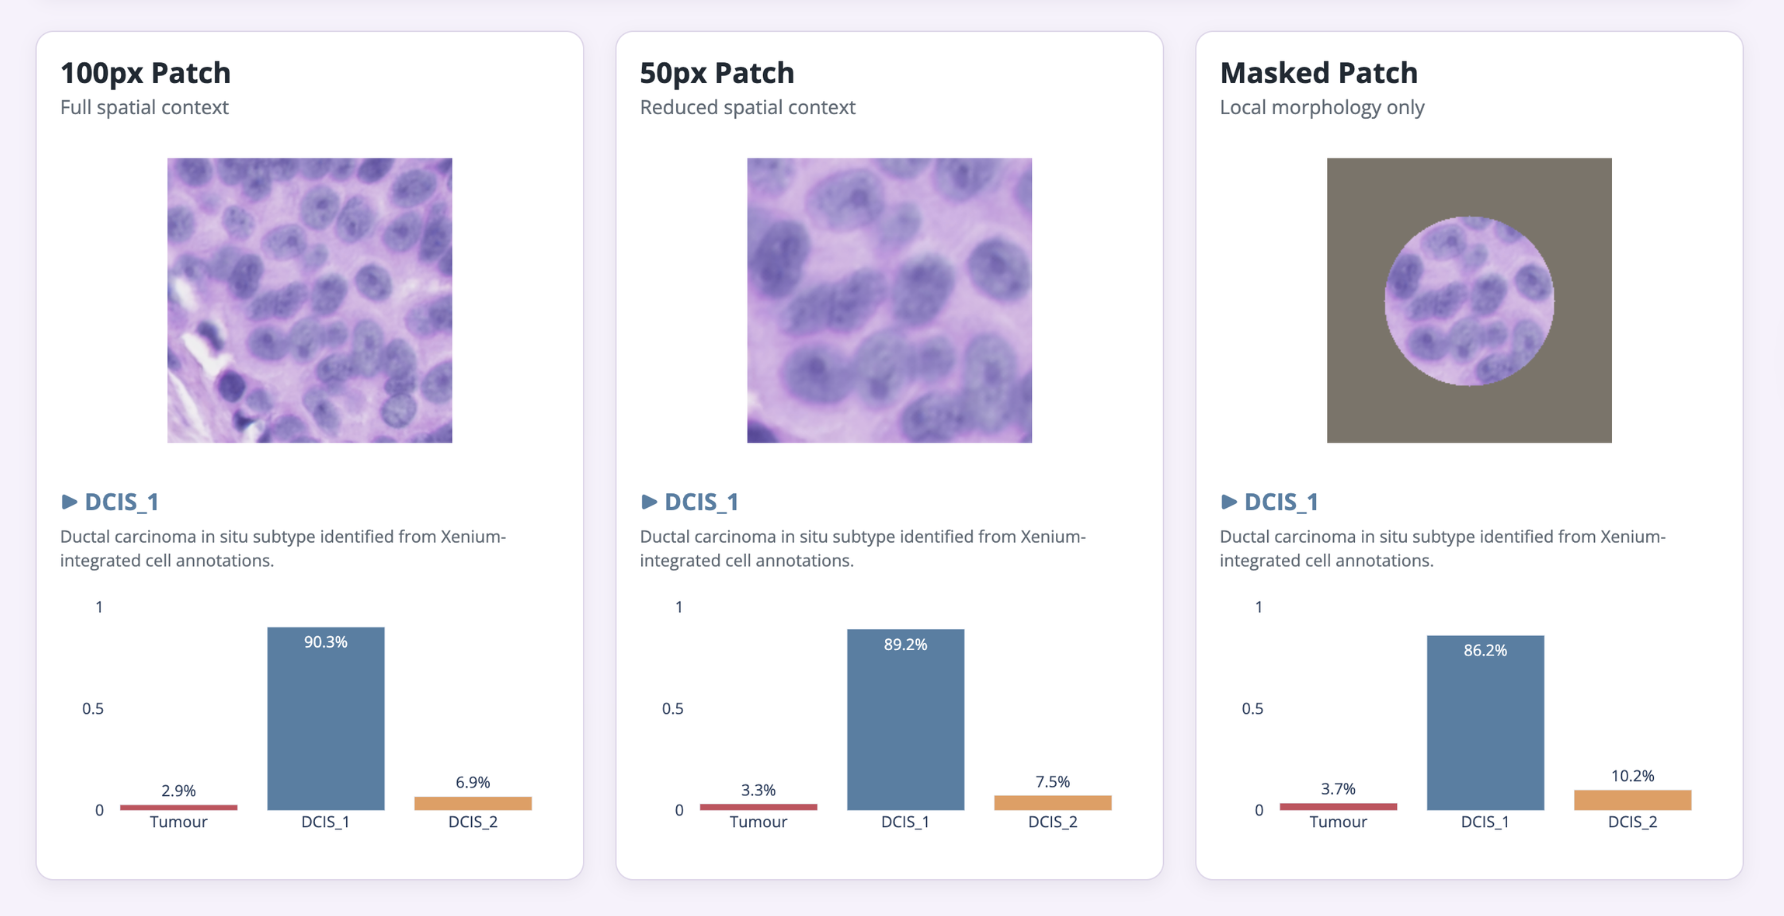
\includegraphics[width=\textwidth]{images/Prediction for cell_10081}
    \caption{Prediction for cell\_10081}
    \label{fig:dc1_tab2}
\end{figure}

\begin{figure}[H]
    \centering
    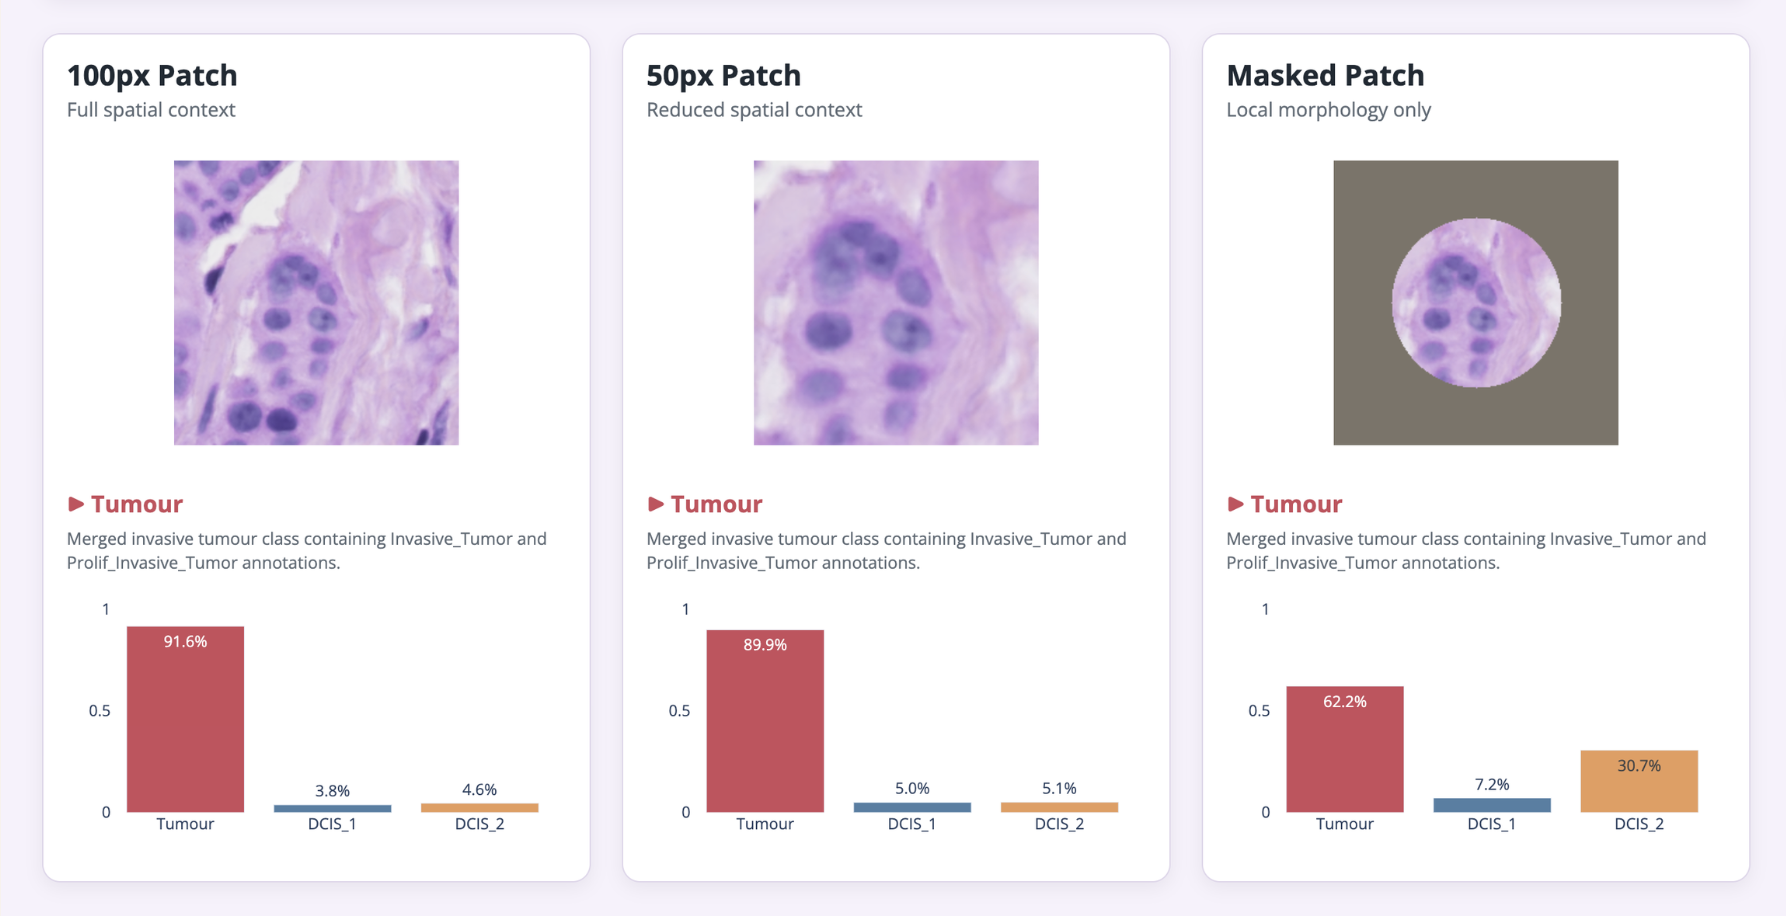
\includegraphics[width=\textwidth]{images/Prediction for cell_100032}
    \caption{Prediction for cell\_100032}
    \label{fig:tum_tab2}
\end{figure}

\begin{figure}[H]
    \centering
    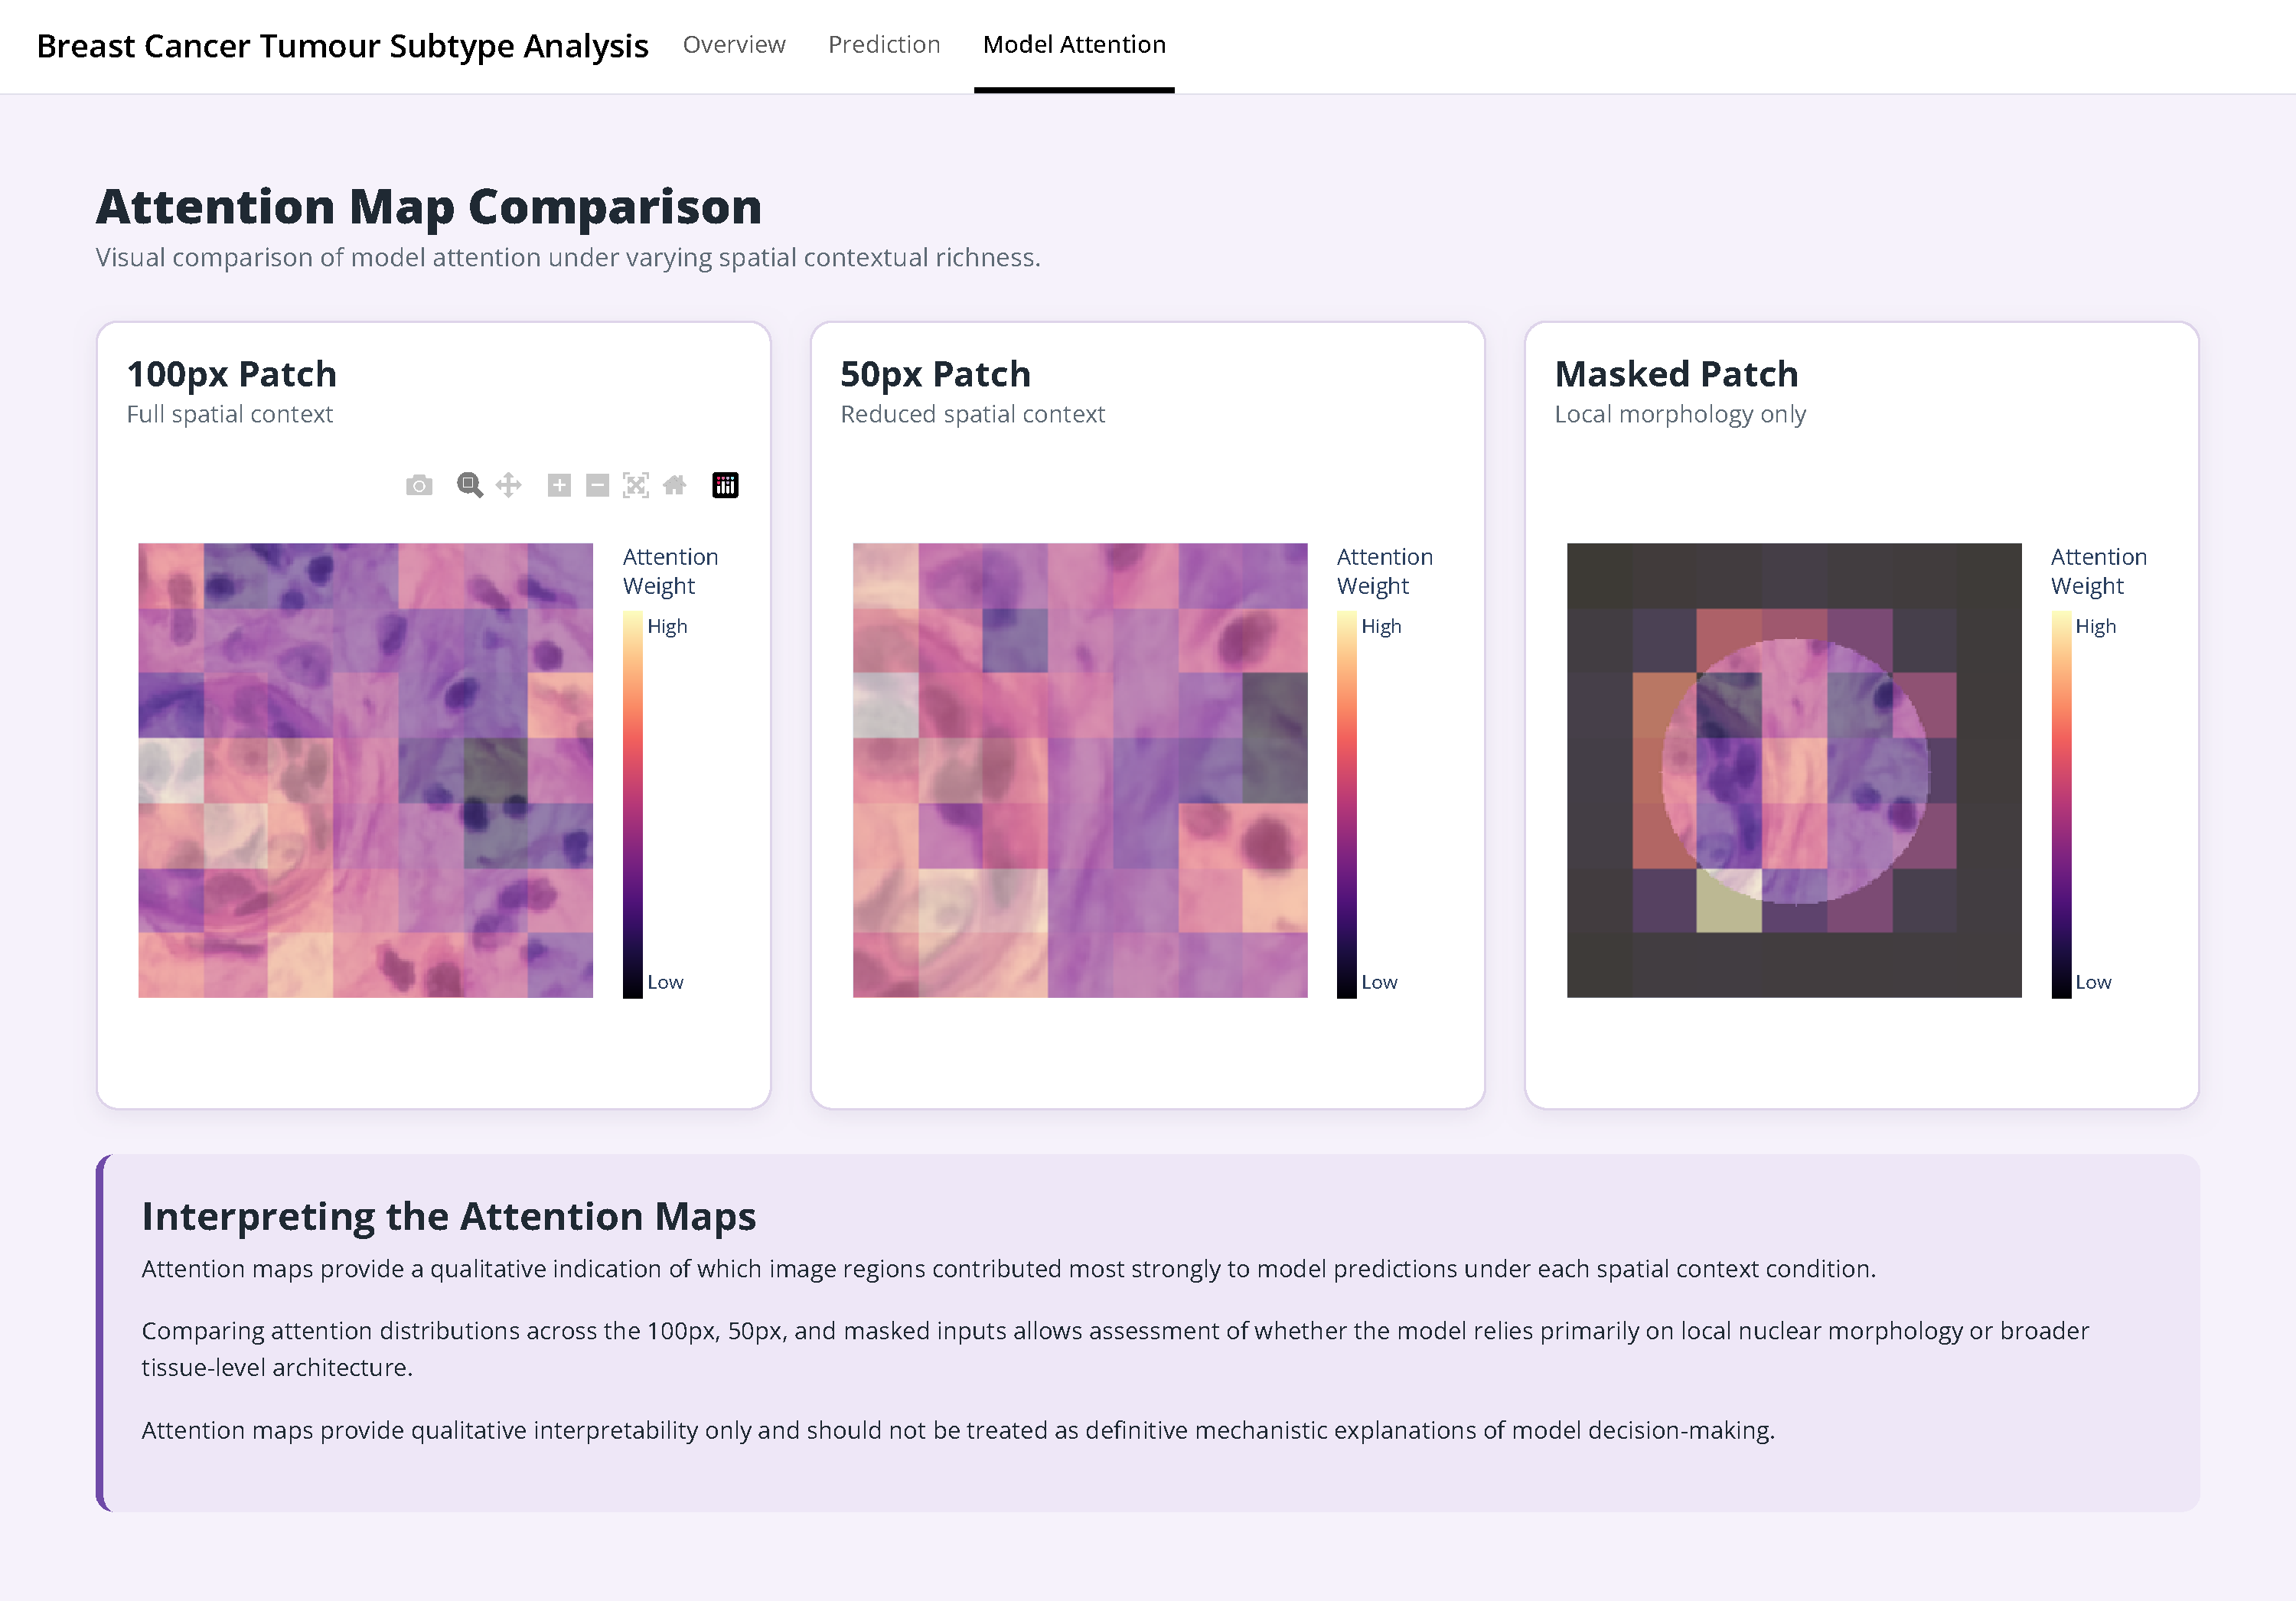
\includegraphics[width=\textwidth]{images/Breast Cancer Tumour Subtype Analysis Model Attention}
    \caption{Tab 3: Side-by-side Attention Map Comparison}
    \label{fig:tab3}
\end{figure}



\end{document}

